\subsection{Workflow Editor Implementation}
The workflow editor interface orchestrates the central canvas, execution logs, and auxiliary tools, providing a cohesive environment for workflow generation and management[cite: 16]. It utilizes a responsive layout with custom absolute positioning, modular popup overlays, and strict state management to track real-time execution lifecycles[cite: 16, 17, 31].

\subsubsection{Main Workflow Page}

\textbf{Purpose:} Acts as the primary application wrapper, housing the interactive header, mode toggles, and state management for the nested editor and AI assistant modules[cite: 16].

\vspace{0.2cm}
\noindent\textbf{Location:} \texttt{WorkflowPage.jsx}[cite: 16]

\vspace{0.2cm}
\noindent\textbf{Components Used:}
\begin{itemize}
    \item \texttt{Chatbot} --- Slide-out drawer component for AI assistance[cite: 16].
    \item \texttt{ExportModal} \& \texttt{ImportModal} --- Overlays managing JSON schema transfers[cite: 16].
    \item \texttt{WorkflowEditor} --- Core canvas component rendering the node-based interface[cite: 16].
\end{itemize}

\vspace{0.2cm}
\noindent\textbf{Notes:}
\begin{itemize}
    \item Implements an interactive breadcrumb header where the workflow name acts as an input field; blurring the input triggers an asynchronous \texttt{PATCH} request to update the project name in the database[cite: 16].
    \item Utilizes CSS absolute positioning paired with a \texttt{transform: translateX(-50\%)} property to perfectly center the "Editor" and "Executions" navigation tabs horizontally across the header[cite: 17].
    \item Maintains dynamic button states for the save function, disabling the button and displaying a loader animation while \texttt{loadSaving} is active, and toggling to a "Saved" visual state upon completion[cite: 16].
\end{itemize}

\begin{figure}[h!]
    \centering
    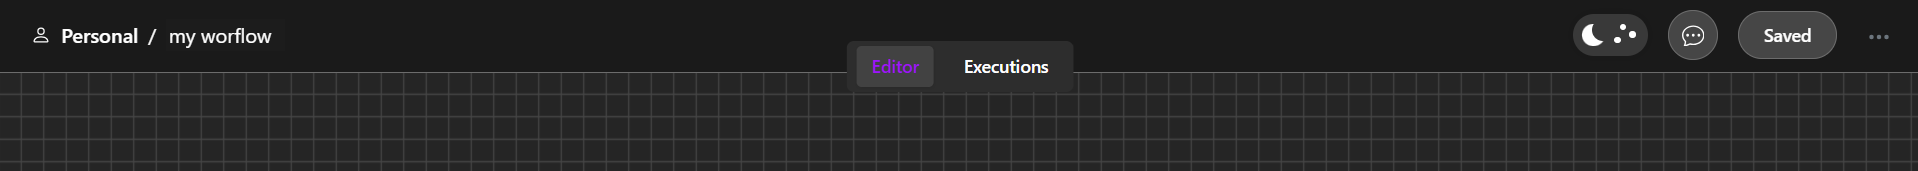
\includegraphics[width=0.95\textwidth]{images/workflow-page/workflow-header-image.png}
    \caption{Header Of Workflow Page Image}
\end{figure}

\subsubsection{Chatbot Assistant Interface}

\textbf{Purpose:} Provides an integrated conversational AI drawer that assists users in building and modifying their workflows via natural language prompts[cite: 18, 19].

\vspace{0.2cm}
\noindent\textbf{Location:} \texttt{Chatbot.jsx}[cite: 19]

\vspace{0.2cm}
\noindent\textbf{Notes:}
\begin{itemize}
    \item Functions as a fixed drawer that slides in from the right viewport edge, smoothly transitioning its \texttt{right} position from \texttt{-400px} to \texttt{0} when toggled open[cite: 18].
    \item Triggers a \texttt{GET} request to \texttt{/api/chat/\{workflowId\}/messages} upon initialization to retrieve and populate historical chat logs[cite: 19].
    \item Renders a dynamic typing indicator during active API calls that cycles through contextual loading steps (e.g., "Analyzing prompt...", "Planning...", "Applying changes...") using a 1500ms interval loop[cite: 19].
\end{itemize}

\begin{figure}[h!]
    \centering
    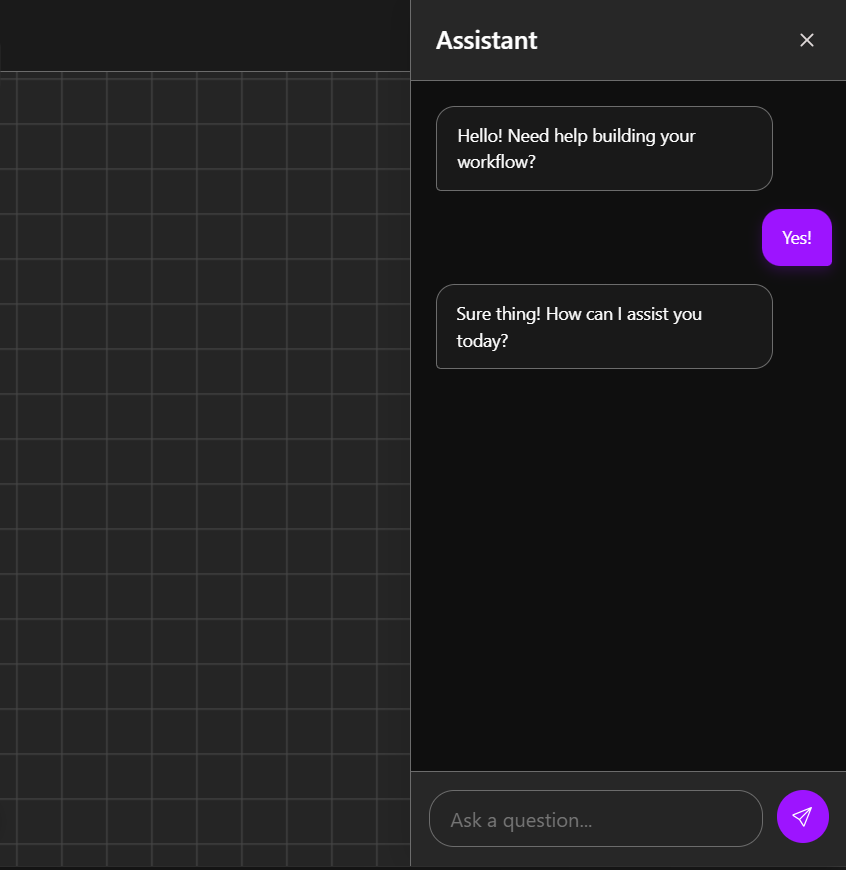
\includegraphics[width=0.43\textwidth]{images/workflow-page/workflow-chatbot-image.png}
    \caption{Chatbot Assistant Interface Image}
\end{figure}

\subsubsection{Workflow Data Management (Import/Export)}

\textbf{Purpose:} Enables the serialization and deserialization of workflow structures into portable JSON formats, facilitating project sharing and backups[cite: 20, 21].

\vspace{0.2cm}
\noindent\textbf{Components:} \texttt{ExportModal.jsx} \& \texttt{ImportModal.jsx}[cite: 16]

\vspace{0.2cm}
\noindent\textbf{Notes:}
\begin{itemize}
    \item \textbf{Exporting:} Invokes a \texttt{GET} request to the \texttt{/export} endpoint and stringifies the returned schema payload with an indentation of 2, displaying it inside a custom scrollable \texttt{textarea}[cite: 21]. Includes a clipboard write integration that temporarily updates the action button to read "Copied!" for 2000ms[cite: 21].
    \item \textbf{Importing:} Safely parses a user-provided JSON string in a \texttt{try/catch} block, specifically extracting \texttt{name}, \texttt{type}, \texttt{description}, \texttt{nodes}, and \texttt{connections} to format the correct \texttt{POST} body[cite: 20].
    \item \textbf{Importing:} Upon successful import, fires a success notification and utilizes \texttt{setTimeout} to force a \texttt{window.location.reload()} after 1000ms to refresh the entire canvas state[cite: 20].
\end{itemize}

\begin{figure}[h!]
    \centering
    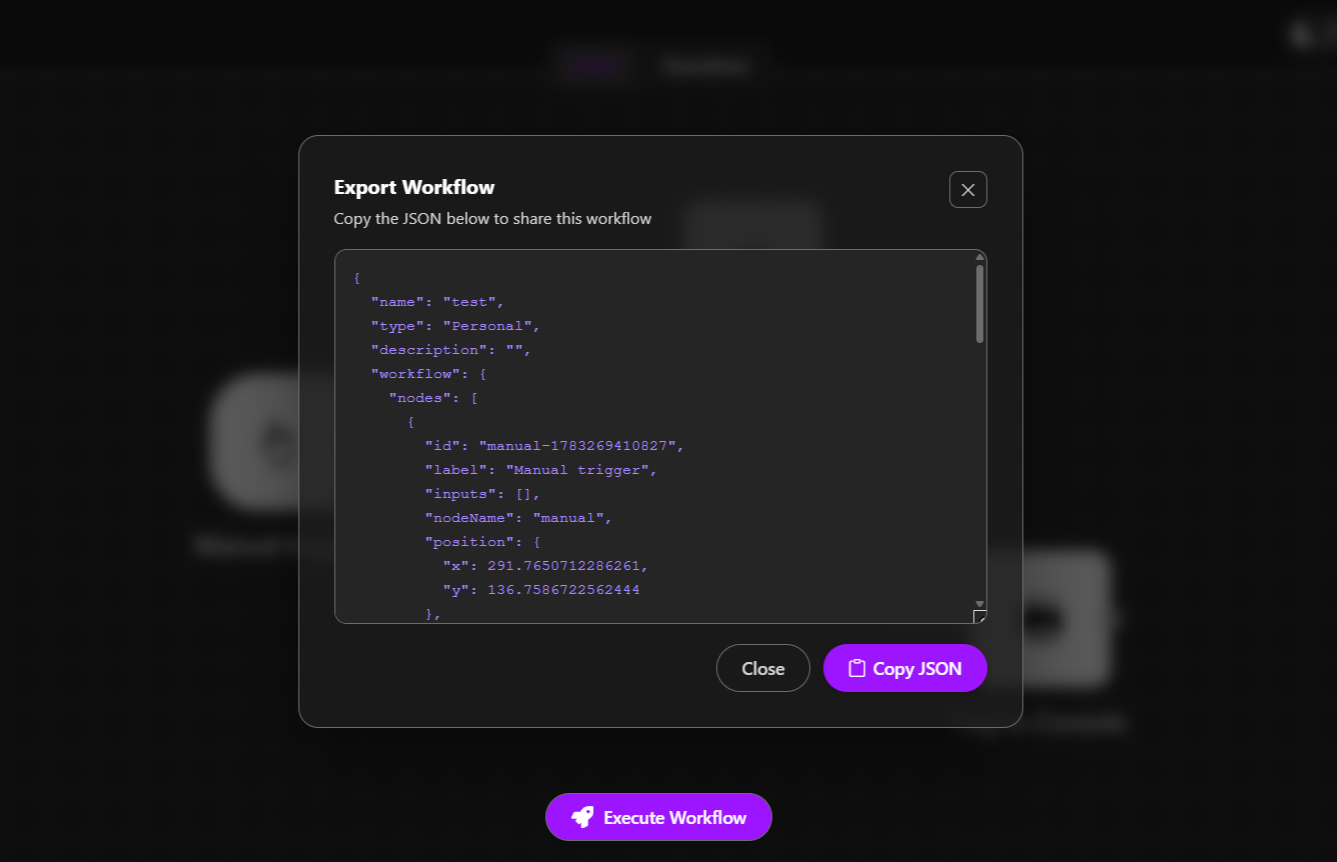
\includegraphics[width=0.95\textwidth]{images/workflow-page/workflow-export-image.png}
    \caption{Workflow Data Management (Export) Image}
\end{figure}
\begin{figure}[h!]
    \centering
    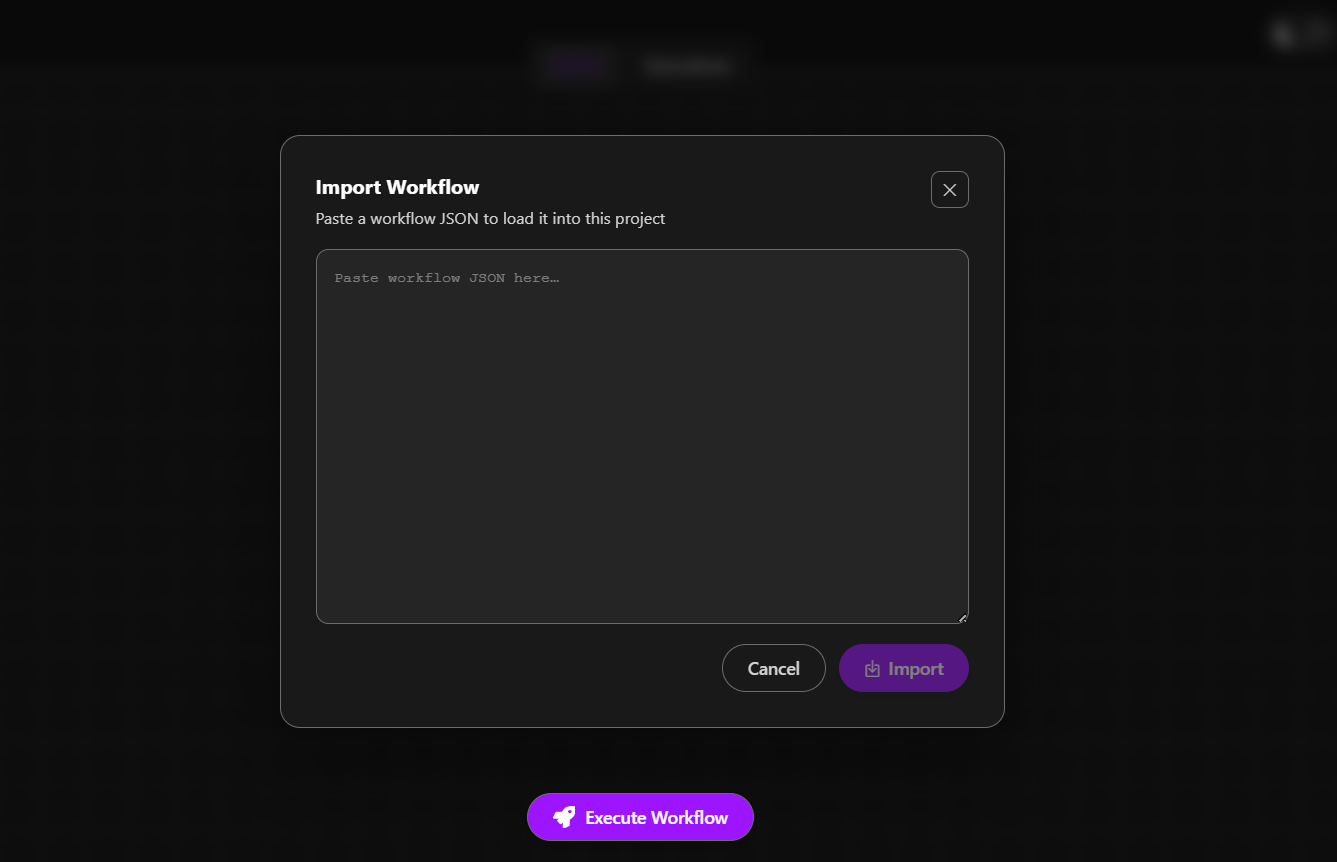
\includegraphics[width=0.95\textwidth]{images/workflow-page/workflow-import-image.png}
    \caption{Workflow Data Management (Import) Image}
\end{figure}

\vspace{0.5cm}

\subsection*{Glassy Navigation Sidebar}

\textbf{Purpose:} Provides a responsive, floating navigation menu with a translucent aesthetic for accessing primary application routes from within the editor.[cite: 27, 28]

\textbf{Location:} \texttt{Sidebar2.jsx}, \texttt{Sidebar2.css}[cite: 27, 28]

\textbf{Components Used:}
\begin{itemize}
    \item \texttt{Link} --- React Router component for managing internal navigation.[cite: 28]
\end{itemize}

\textbf{Notes:}
\begin{itemize}
    \item Utilizes the \texttt{backdrop-filter: blur(10px)} property alongside a translucent background to create a frosted-glass visual aesthetic layered over the canvas.[cite: 27]
    \item Houses core navigation routes directing the user to the Overview, Workflow Creation, and User Profile pages.[cite: 28]
    \item Features a hover-expand interaction where lingering on a default icon triggers a \texttt{hover-pill} container to smoothly transition its width and opacity, revealing the full navigational text label.[cite: 27, 28]
    \item Includes a responsive media query that shrinks the overall sidebar footprint and outright disables the expanding hover pills on mobile displays \texttt{(max-width: 400px)} to prevent interface overlapping.[cite: 27]
\end{itemize}

\begin{figure}[h!]
    \centering
    
\includegraphics[width=0.7\textwidth]{images/workflow-page/workflow-sidebar-image.png}
    \caption{Glassy Navigation Sidebar Image}
\end{figure}

\subsubsection{Main Flow Editor Component}

\textbf{Purpose:} Acts as the central interactive canvas mapping node coordinates, handling connection logic, and managing real-time auto-saving diffs.

\vspace{0.2cm}
\noindent\textbf{Location:} \texttt{FlowEditor.jsx}[cite: 31]

\vspace{0.2cm}
\noindent\textbf{Components Used:}
\begin{itemize}
    \item \texttt{ReactFlow} --- Core framework component for rendering customizable nodes and edges[cite: 31].
    \item \texttt{NodesPanel} --- Interface panel for dragging and dropping new nodes onto the workspace[cite: 31].
    \item \texttt{NodeParameterPopup} --- Modal for configuring specific node inputs, API parameters, and authentication credentials[cite: 31].
\end{itemize}

\vspace{0.2cm}
\noindent\textbf{Notes:}
\begin{itemize}
    \item Manages the complex serialization of the visual workflow into a strict JSON payload that accurately captures node coordinates, custom labels, configuration parameters, and edge mapping[cite: 31].
    \item Maintains a stringified snapshot of the initial canvas state (\texttt{savedSnapshotRef}) to continuously diff against current changes, accurately updating the "Unsaved Changes" indicator in real-time[cite: 31].
    \item Handles asynchronous API requests to persist modifications via \texttt{PATCH} requests and restores previous project configurations upon initial mount via \texttt{GET} requests[cite: 31].
\end{itemize}

\subsubsection{Custom Node Interfaces}

\textbf{Purpose:} Replaces default canvas nodes with interactive custom DOM structures that support execution animations, specific connection logic, and in-place renaming[cite: 25, 30].

\vspace{0.2cm}
\noindent\textbf{Location:} \texttt{NormalNode.jsx}[cite: 25], \texttt{TriggerNode.jsx}[cite: 30], \texttt{RenameModal.jsx}[cite: 26]

\vspace{0.2cm}
\noindent\textbf{Notes:}
\begin{itemize}
    \item Differentiates between standard processing nodes (featuring both target and source handles for sequential linking) and trigger nodes (featuring exclusively a right-side source handle to initiate flows)[cite: 25, 30].
    \item Embeds absolute-positioned modifier buttons (trash and pencil icons) for deletion and renaming; these remain hidden and purposefully disable pointer events until the parent container is actively hovered to maintain a clean aesthetic[cite: 25, 29, 30].
    \item Renaming intercepts user input via the \texttt{RenameModal} to visually update the \texttt{label} property while strictly preserving the underlying technical \texttt{nodeName} required for backend processing[cite: 25, 26, 30].
    \item During an active execution phase (\texttt{RUNNING} state), actively processing nodes receive a \texttt{node-running} class that triggers a CSS \texttt{@keyframes} animation, producing a continuous pulsing shadow effect[cite: 24, 25, 29, 30].
\end{itemize}

\begin{figure}[h!]
    \centering
    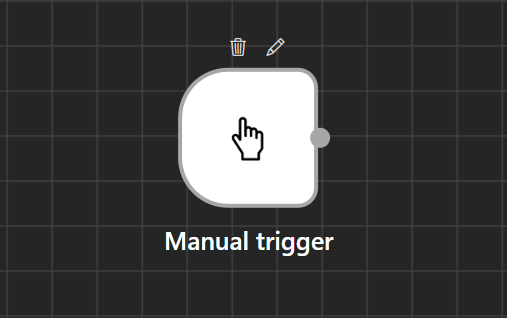
\includegraphics[width=0.65\textwidth]{images/workflow-page/workflow-node-image.png}
    \caption{Custom Node Interfaces Image}
\end{figure}

\subsubsection{Dynamic Edge Connections}

\textbf{Purpose:} Renders visual paths between nodes, incorporating interactive deletion overlays and animated states to reflect active data movement[cite: 23].

\vspace{0.2cm}
\noindent\textbf{Location:} \texttt{CustomEdge.jsx}[cite: 23], \texttt{CustomEdge.css}[cite: 22]

\vspace{0.2cm}
\noindent\textbf{Notes:}
\begin{itemize}
    \item Calculates a smooth bezier curve path between node handles rather than utilizing standard straight or stepped connection lines[cite: 23].
    \item Embeds an SVG \texttt{foreignObject} exactly at the midpoint of the calculated path, rendering a hidden delete button that becomes interactive and fully opaque only when the edge group is hovered by the cursor[cite: 22, 23].
    \item When the workflow execution status shifts to \texttt{RUNNING}, edges render an additional animated flowing overlay[cite: 23]. This utilizes \texttt{stroke-dasharray} and \texttt{stroke-dashoffset} keyframes to create a dashed line that continuously moves along the path[cite: 22].
\end{itemize}

\begin{figure}[h!]
    \centering
    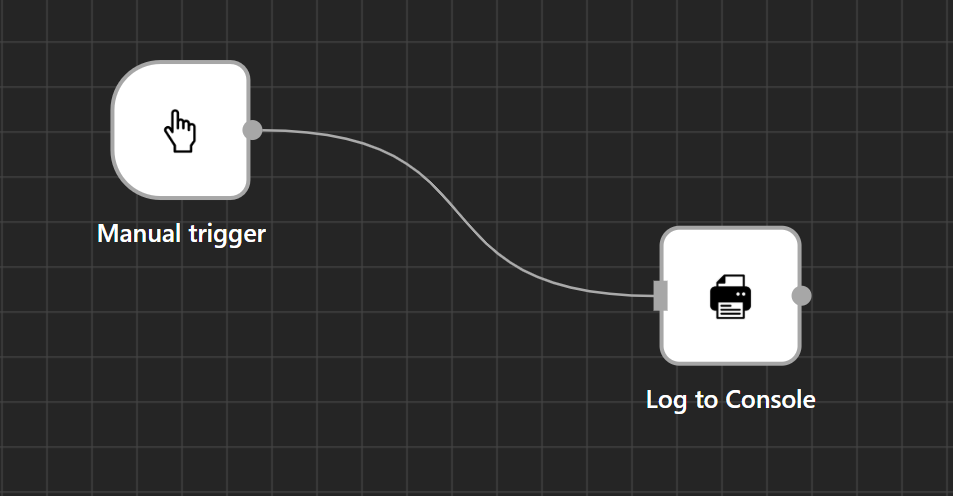
\includegraphics[width=0.55\textwidth]{images/workflow-page/workflow-nedge-image.png}
    \caption{Dynamic Edge Connections (Default state) Image}
\end{figure}
\begin{figure}[h!]
    \centering
    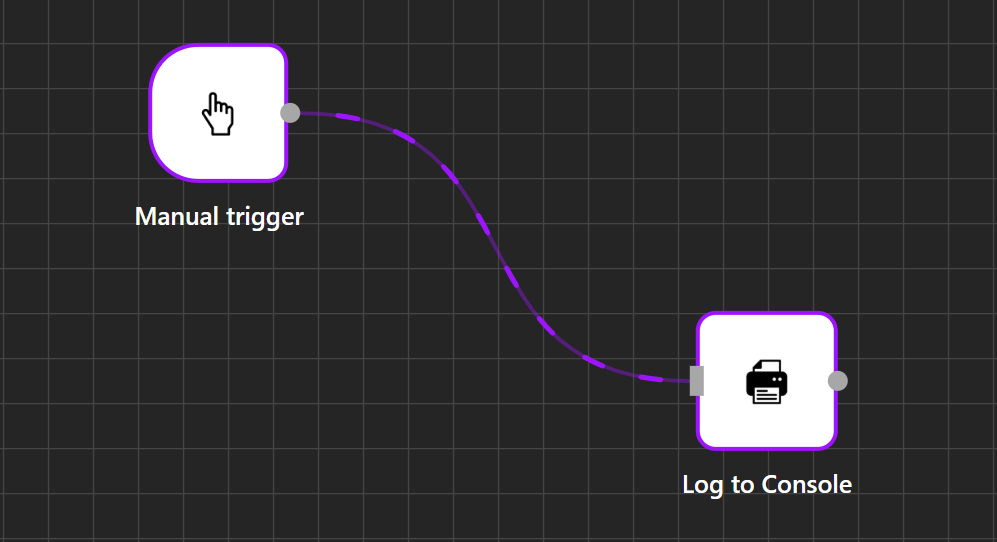
\includegraphics[width=0.55\textwidth]{images/workflow-page/workflow-redge-image.png}
    \caption{Dynamic Edge Connections (RUNNING state) Image}
\end{figure}

\subsubsection{Execution and Lifecycle Controls}

\textbf{Purpose:} Manages the active invocation and termination of workflow sequences, providing immediate visual feedback and locking canvas mutations during active runs.

\vspace{0.2cm}
\noindent\textbf{Location:} \texttt{FlowEditor.jsx}[cite: 31]

\vspace{0.2cm}
\noindent\textbf{Notes:}
\begin{itemize}
    \item Tracks and controls execution states explicitly using an enumerated status mapping: \texttt{IDLE}, \texttt{PENDING}, \texttt{RUNNING}, and \texttt{STOPPING}[cite: 31].
    \item Dynamically swaps the primary action button based on the state. If the workflow is \texttt{IDLE}, an "Execute" button is rendered. During \texttt{RUNNING}, it is replaced by a pink "Stop Execution" button, and during transitionary states (\texttt{PENDING}, \texttt{STOPPING}), it renders disabled loading indicators[cite: 31].
    \item Hitting the execution button aggregates the current canvas schema via the \texttt{savedSnapshotRef} and dispatches it to the backend engine, while hitting stop sends an abort signal to gracefully halt node processing[cite: 31].
\end{itemize}

\begin{lstlisting}
// Example logic derived from FlowEditor.jsx state management
const renderExecutionControls = () => {
  switch (executionStatus) {
    case 'IDLE':
      return (
        <button onClick={handleExecute} className="btn-execute">
          <PlayIcon /> Execute Workflow
        </button>
      );
    case 'PENDING':
      return (
        <button disabled className="btn-loading">
          <Spinner /> Starting...
        </button>
      );
    case 'RUNNING':
      return (
        <button onClick={handleStop} className="btn-stop">
          <StopIcon /> Stop Execution
        </button>
      );
    case 'STOPPING':
      return (
        <button disabled className="btn-loading">
          <Spinner /> Stopping...
        </button>
      );
    default:
      return null;
  }
};
\end{lstlisting}

%%%%%%%%%%%%%%%%%%%%%%%%%%%%%%%%%%%%%%%%%%%%%%%%%%%%%%%%
%%%  NODE PANEL PART ------ SARA -------  %%%
%%%%%%%%%%%%%%%%%%%%%%%%%%%%%%%%%%%%%%%%%%%%%%%%%%%%%%%%

\subsection*{NodeParameterPopup Component}

\textbf{Purpose:} Renders a modal popup for configuring a workflow node --- allowing users to set input source, parameters, and credentials before saving and executing the node.

\textbf{Location:} \texttt{src/pages/Workflow/components/NodeParameterPopup.jsx}

\textbf{Props:}
\begin{itemize}
    \item \texttt{node} (Object) --- The selected workflow node, containing its data, parameters, credentials, and saved inputs.
    \item \texttt{open} (Boolean) --- Controls modal visibility.
    \item \texttt{onClose} (Function) --- Callback to close the modal.
    \item \texttt{onSave} (Function) --- Callback invoked with the node's updated parameters, credentials, inputs, and input source on save.
\end{itemize}

\textbf{Layout --- Three-Panel Structure:}
\begin{itemize}
    \item \textbf{Left Panel (Node Input):} Lets the user choose an input source (self, parent, or combined). When self or combined is selected, renders the appropriate input control based on \texttt{inputFormat.type}: a file/image uploader, a JSON array textarea with live validation, or a plain text field. If the node has no \texttt{inputFormat}, a "no input required" message is shown instead.
    \item \textbf{Center Panel (Parameters / Credentials):} Contains a \texttt{PopupHeader} with tab navigation and a body that switches between \texttt{ParameterForm} (node configuration fields) and \texttt{CredentialsForm} (authentication fields including OAuth).
    \item \textbf{Right Panel (Node Output):} Displays the node's \texttt{outputDescription} if defined.
\end{itemize}

\textbf{Behavior:}
\begin{itemize}
    \item On open, restores the node's previously saved \texttt{inputSource} and inputs into the appropriate input state (files, JSON, or text).
    \item After an OAuth redirect, restores the active tab from \texttt{localStorage} and saves \texttt{formData} to \texttt{localStorage} before the redirect occurs.
    \item On save (\texttt{handleExecute}), collects and validates inputs via \texttt{buildInputs()}, merges them with parameters and credentials, calls \texttt{onSave}, then closes the modal. Throws inline alerts on validation errors (e.g., malformed JSON).
    \item File uploads and deletions are handled via \texttt{NodeService.uploadFiles()} and \texttt{NodeService.deleteFile()}, with per-file loading states for both uploading and deletion.
    \item Wraps the modal with an \texttt{Overlay} component and a back button for closing.
\end{itemize}

\textbf{Hooks Used:}
\begin{itemize}
    \item \texttt{useNodeParameters} --- Manages parameter form state, date/time conversion utilities, and parameter serialization.
    \item \texttt{useNodeCredentials} --- Manages credentials form state, OAuth flow, and credentials serialization.
\end{itemize}

\vspace{0.5cm}

\subsection*{useNodeParameters Hook}

\textbf{Purpose:} Manages the parameter form state for a workflow node, including initialization from saved or default values, field change handling, and serialization before save.

\textbf{Location:} \texttt{src/hooks/useNodeParameters.js}

\textbf{Parameters:}
\begin{itemize}
    \item \texttt{node} (Object) --- The selected workflow node containing raw parameter definitions and previously saved parameter values.
\end{itemize}

\textbf{Returns:} \texttt{formData}, \texttt{setFormData}, \texttt{handleChange}, \texttt{timestampToDatetimeLocal}, \texttt{datetimeLocalToTimestamp}, \texttt{prepareParametersForSave}

\textbf{Behavior:}
\begin{itemize}
    \item On node change, initializes \texttt{formData} by merging saved parameter values with raw parameter definitions, falling back to defaults where no saved value exists. Applies type coercion for timestamp (stored as a number) and number fields.
    \item If returning from an OAuth redirect, overrides the initialized \texttt{formData} with the value stored in \texttt{localStorage} (\texttt{oauth\_return\_formData}), then clears it.
    \item \texttt{handleChange} updates a single field in \texttt{formData} by key.
    \item \texttt{timestampToDatetimeLocal} and \texttt{datetimeLocalToTimestamp} convert between Unix timestamps and datetime-local input format for datetime fields.
    \item \texttt{prepareParametersForSave} serializes \texttt{formData} into a typed array (title, type, value) suitable for the backend, applying type coercion for timestamp, number, and toggle fields.
\end{itemize}

\begin{figure}[h!]
    \centering
    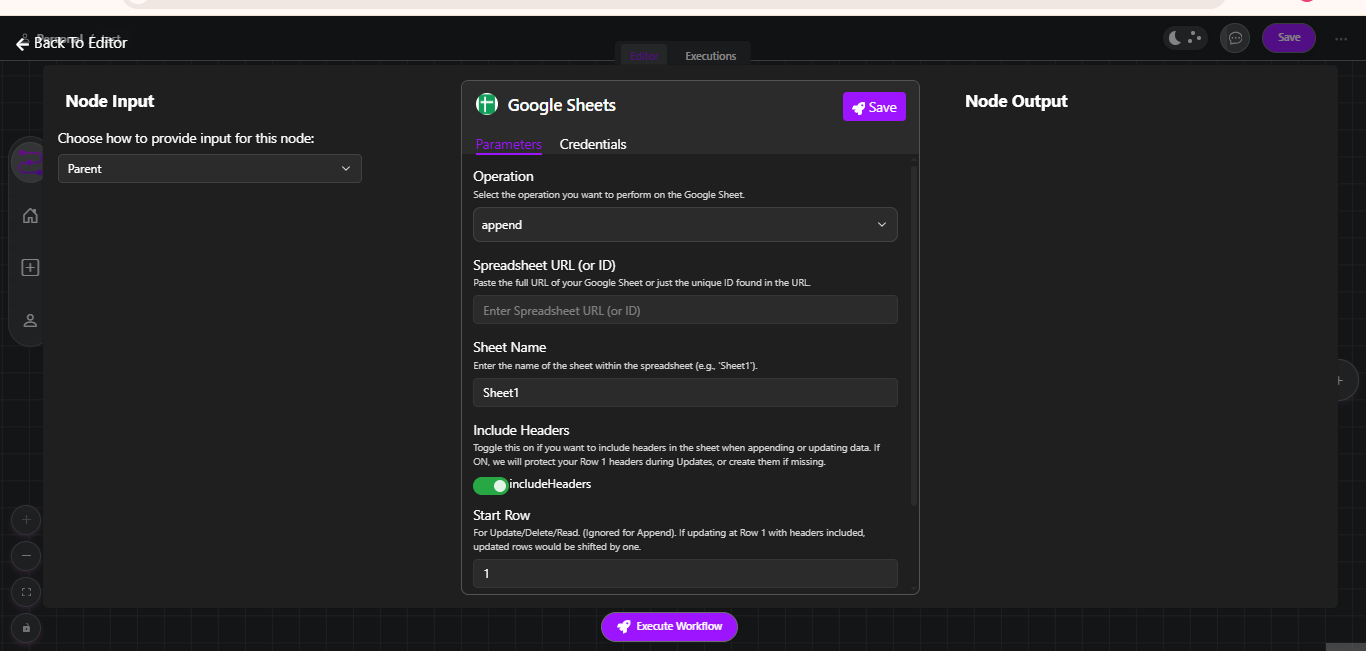
\includegraphics[width=0.6\textwidth]{images/workflow-page/workflow-params-image.png}
    \caption{Node Parameters Image}
\end{figure}

\vfill
\hrule
\vspace{0.5cm}

\subsection*{useNodeCredentials Hook}

\textbf{Purpose:} Manages credential selection state for a workflow node, including fetching available credential types and sets, handling saved credential restoration, and initiating the OAuth flow.

\textbf{Location:} \texttt{src/hooks/useNodeCredentials.js}

\textbf{Parameters:}
\begin{itemize}
    \item \texttt{node} (Object) --- The selected workflow node containing credential type references and previously saved credential selections.
    \item \texttt{setAuth} (Object) --- Global auth context passed to service calls.
\end{itemize}

\textbf{Returns:} \texttt{credentialsData}, \texttt{credentialsFormData}, \texttt{handleChangedentials}, \texttt{prepareCredentialsForSave}, \texttt{handleOAuthClick}, \texttt{isLoadingCredentials}

\textbf{Behavior:}
\begin{itemize}
    \item On mount, fetches each required credential type and its available credential sets via \texttt{CredentialService}, then restores previously saved selections from the node or falls back to empty.
    \item Listens for the \texttt{oauthCredentialsReload} window event (dispatched by \texttt{WorkflowEditor} after an OAuth redirect) to reload credentials and auto-select the newly created set identified by \texttt{localStorage} (\texttt{oauth\_return\_credTitle}).
    \item \texttt{handleChangedentials} updates a single credential selection by key.
    \item \texttt{prepareCredentialsForSave} serializes selected credentials into \{ \texttt{typeId}, \texttt{setId} \} pairs for the backend.
    \item \texttt{handleOAuthClick} saves the current node state, active tab, and credential title to \texttt{localStorage}, dispatches \texttt{beforeOAuthRedirect} to trigger a workflow save, then redirects the browser to the Google OAuth URL with the project ID and access token as query parameters.
\end{itemize}

\begin{figure}[h!]
    \centering
    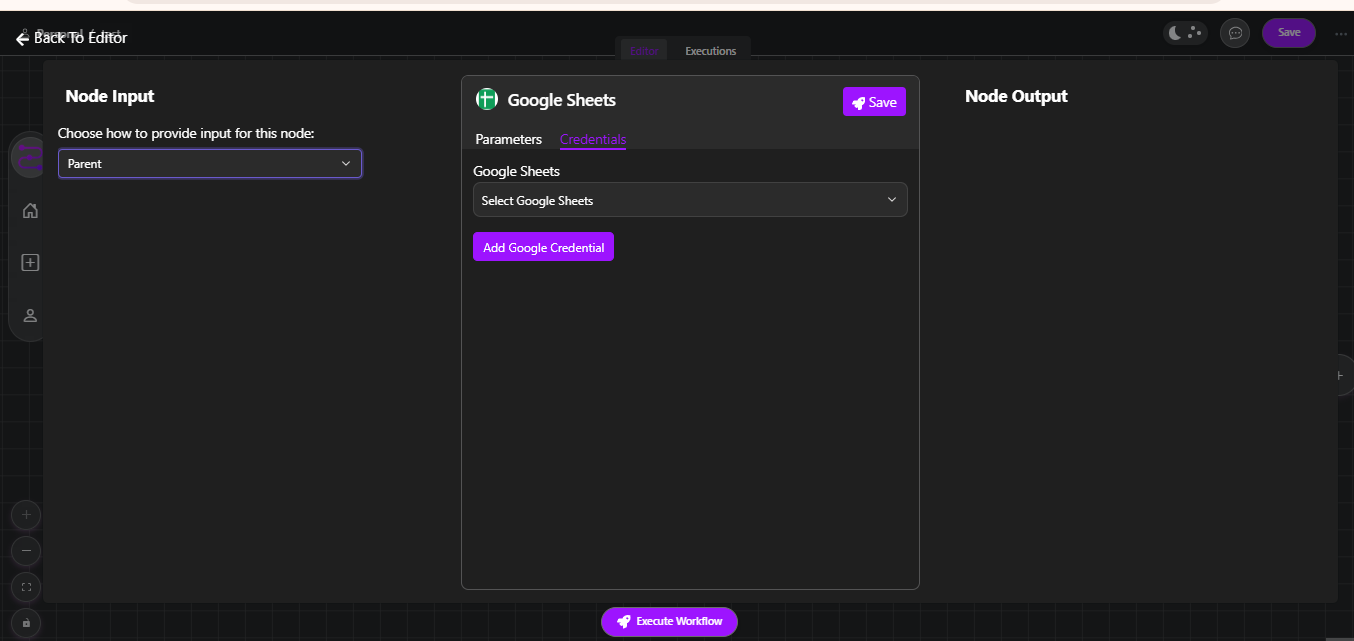
\includegraphics[width=0.6\textwidth]{images/workflow-page/workflow-creds-image.png}
    \caption{Node Credentials Image}
\end{figure}

\vfill
\hrule
\vspace{0.5cm}

\subsection*{Node Parameter Popup --- Left Panel (Node Input)}

\textbf{Purpose:} Allows the user to configure how the node receives its input, driven entirely by the node's \texttt{inputFormat} definition.

\textbf{Behavior:}
\begin{itemize}
    \item \textbf{Input Source Selector:} If the node has an \texttt{inputFormat}, a dropdown lets the user choose from three sources:
    \begin{itemize}
        \item \textbf{self} --- the user provides the input directly.
        \item \textbf{parent} --- input is inherited from the preceding node; no input field is shown.
        \item \textbf{combined} --- the user provides additional input alongside the parent's output.
    \end{itemize}
    \item \textbf{Input Controls:} When self or combined is selected, an input field is rendered based on \texttt{inputFormat.type}:
    \begin{itemize}
        \item \textbf{File / Image} (\texttt{type: "file"} or \texttt{"image"}): Renders a drag-and-drop upload box respecting \texttt{inputFormat.accept} and \texttt{inputFormat.multiple}. Files upload immediately via \texttt{NodeService.uploadFiles()}. Uploaded files display as cards --- images show a thumbnail preview, non-image files show a document icon, each linking to the file in a new tab. Each card has a delete button that calls \texttt{NodeService.deleteFile()} with a per-file spinner; restored files (prefixed \texttt{restored-}) are removed locally without an API call. On restore, saved URLs are labeled "Image N" or "File N" since raw URLs don't carry readable filenames.
        \item \textbf{JSON} (\texttt{type: "json"}): Renders a textarea expecting a JSON array of objects (e.g., \texttt{[\{"key":"value"\}]}). Live validation runs on every keystroke via \texttt{validateJsonArray}, checking for valid JSON, array structure, and that every item is a non-null object, with errors shown inline. On save, input is re-validated, parsed, and stored as a normalized JSON string.
        \item \textbf{Text / Any} (default): Renders a plain text input field for any other input type.
    \end{itemize}
    \item \textbf{No Input:} If the node has no \texttt{inputFormat}, a "This node does not require any input" message is shown instead.
\end{itemize}

\begin{figure}[H]
    \centering
    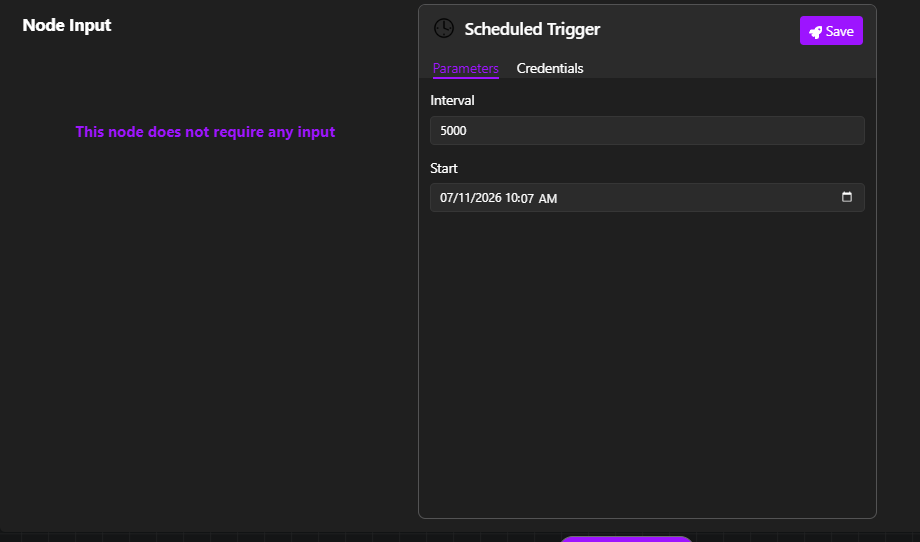
\includegraphics[width=0.6\textwidth]{images/workflow-page/workflow-input1-image.png}
    \caption{Node Input Type 1 Image}
\end{figure}
\begin{figure}[H]
    \centering
    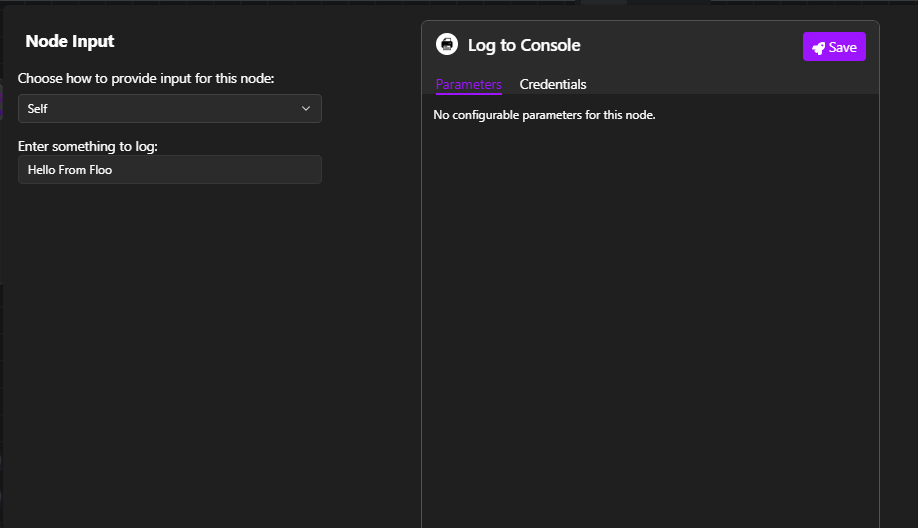
\includegraphics[width=0.6\textwidth]{images/workflow-page/workflow-input2-image.png}
    \caption{Node Input Type 2 Image}
\end{figure}
\begin{figure}[H]
    \centering
    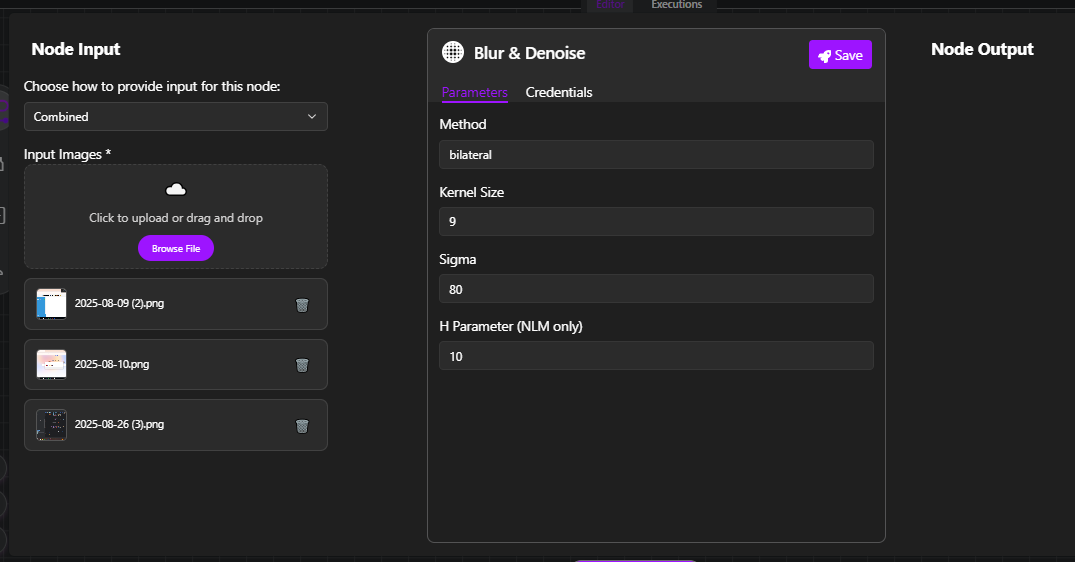
\includegraphics[width=0.6\textwidth]{images/workflow-page/workflow-input3-image.png}
    \caption{Node Input Type 3 Image}
\end{figure}
\begin{figure}[H]
    \centering
    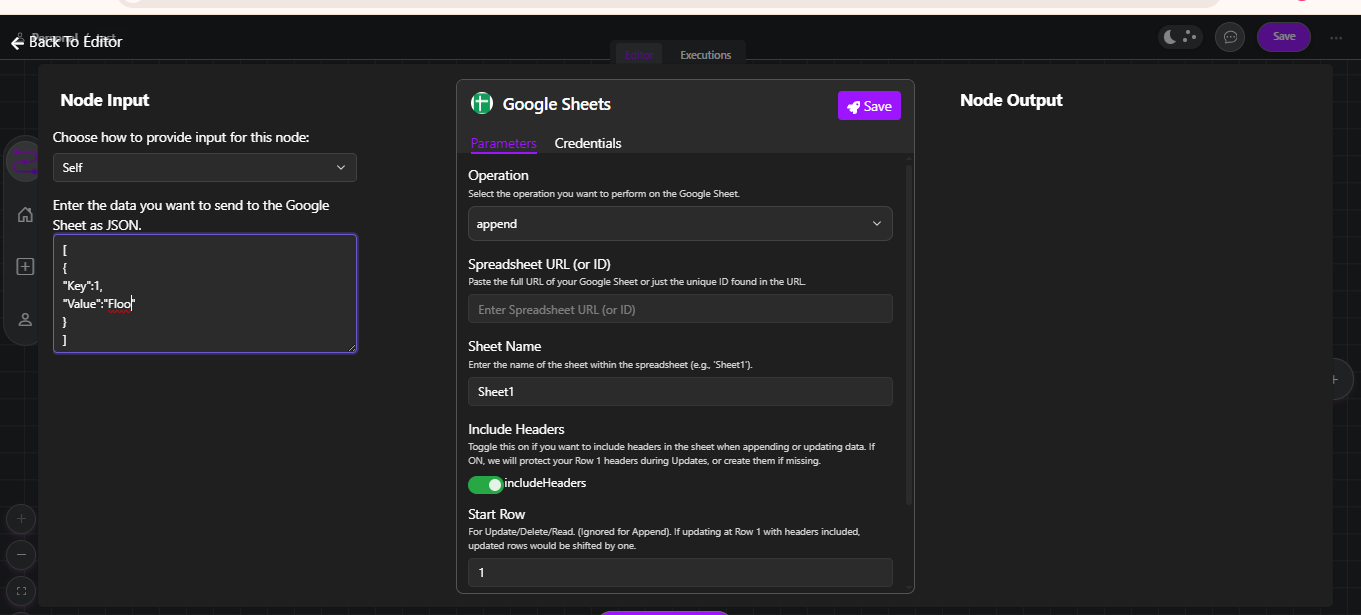
\includegraphics[width=0.6\textwidth]{images/workflow-page/workflow-input4-image.png}
    \caption{Node Input Type 4 Image}
\end{figure}
\begin{figure}[H]
    \centering
    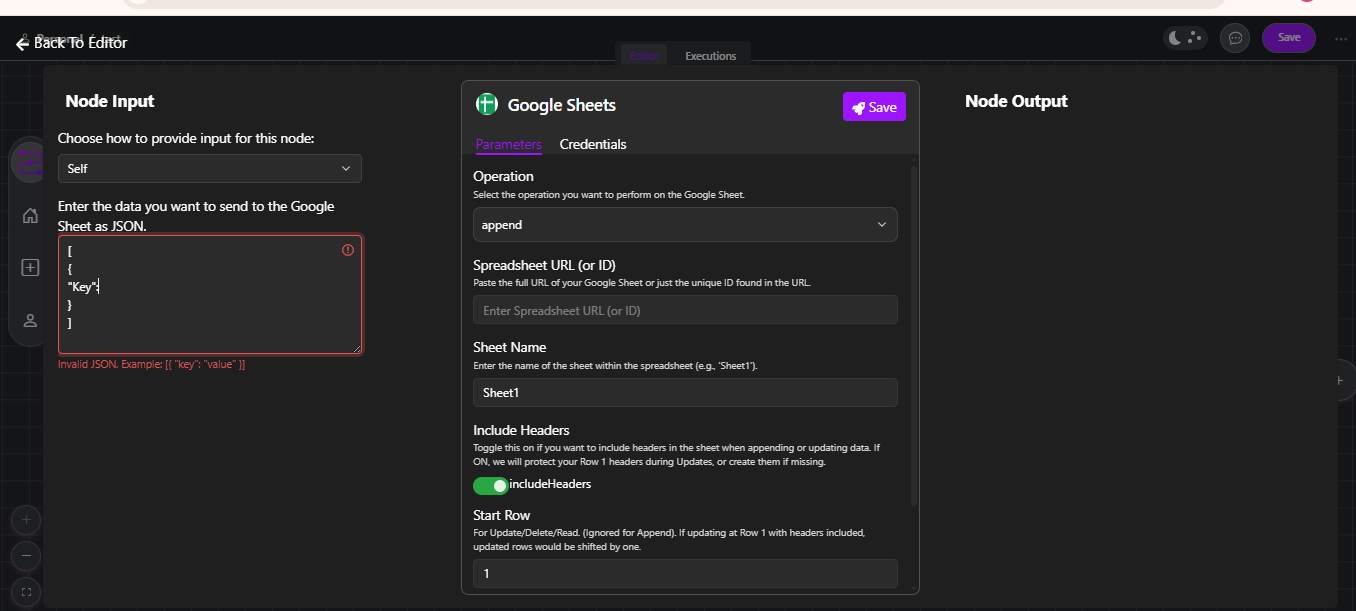
\includegraphics[width=0.6\textwidth]{images/workflow-page/workflow-input5-image.png}
    \caption{Node Input Type 5 Image}
\end{figure}

\vspace{0.9cm}
\subsection*{Execution History Sidebar Component}

\textbf{Purpose:} Renders a slide-in sidebar panel displaying the workflow's historical execution logs for the current project when the Executions tab is engaged.

\vspace{0.2cm}
\noindent\textbf{Location:} \texttt{src/pages/Workflow/components/ExecutionsSidebar.jsx}

\vspace{0.2cm}
\noindent\textbf{Props:}
\begin{itemize}
    \item \texttt{isOpen} (Boolean) --- Controls sidebar visibility; returns \texttt{null} and stops active data polling when set to \texttt{false}.
\end{itemize}

\vspace{0.2cm}
\noindent\textbf{Components Used:}
\begin{itemize}
    \item \texttt{ExecutionsList} --- Renders the full list of executions with output previews, status icons, structured output badges, a lightbox viewer, and download controls.
\end{itemize}

\vspace{0.2cm}
\noindent\textbf{Notes:}
\begin{itemize}
    \item Resolves the project ID dynamically from URL parameters via \texttt{useParams}, gracefully falling back to \texttt{useProjectContext} if unavailable.
    \item Delegates all complex execution data retrieval and state management to the \texttt{useExecutions} custom hook, passing the refined results directly to the \texttt{ExecutionsList}.
    \item Displays a specialized panel header titled "Executions" containing a dynamic count badge when executions are available and not in a loading state.
    \item Renders nothing when \texttt{isOpen} is false, which intentionally pauses the background polling interval to preserve client memory and network bandwidth.
\end{itemize}

\subsubsection{Executions List Component}

\textbf{Purpose:} Renders the comprehensive list of execution records inside the sidebar. Each record displays start/finish timestamps, status indicators, structured-output badges, raw-output previews, and a dedicated lightbox viewer.

\vspace{0.2cm}
\noindent\textbf{Location:} \texttt{src/pages/Workflow/components/ExecutionsList.jsx}

\vspace{0.2cm}
\noindent\textbf{Props:}
\begin{itemize}
    \item \texttt{executions} (Array) --- The execution records mapped for display.
    \item \texttt{selectedExecution} (Object | null) --- The currently active execution, which receives a selected visual highlight.
    \item \texttt{expandedOutputs} (Set) --- Tracks IDs of executions whose raw output blocks are expanded.
    \item \texttt{onSelectExecution} (Function) --- Callback invoked when a specific execution card is clicked.
    \item \texttt{onToggleOutput} (Function) --- Callback invoking raw output expansion/collapse.
    \item \texttt{getOutputPreview}, \texttt{shouldShowToggle}, \texttt{getStatusIcon}, \texttt{getStructuredOutputs} (Functions) --- Utility handlers passed down from the hook for string truncation, visual mapping, and data grouping.
    \item \texttt{forceDownload} (Function) --- Utility to trigger external asset downloads.
    \item \texttt{loading} (Boolean) \& \texttt{error} (String | null) --- Interface state flags.
\end{itemize}

\vspace{0.2cm}
\noindent\textbf{Behavior:}
\begin{itemize}
    \item Short-circuits the render cycle to display a loading indicator, an error message, or a fallback "No executions found" state based on the hook's returned flags.
    \item Evaluates each execution through \texttt{getStructuredOutputs} to count distinct assets (Images, Files, JSON, Text), selectively rendering clickable visual badges when items are present.
    \item Conditionally renders raw-output blocks when the execution yields text, triggers an error/failed status, or lacks structured assets entirely. Accompanied by a "Show more / less" toggle.
    \item Clicking a card selects the execution; clicking the output toggles the expansion state; clicking an asset badge opens the isolated lightbox view.
    \item The embedded lightbox modal iterates through each asset per node, applying a type-specific renderer (image preview, raw file path, or pretty-printed JSON) alongside a direct \texttt{Download} button action.
\end{itemize}

\subsubsection{Executions Data Logic (\texttt{useExecutions} Hook)}

\textbf{Purpose:} Encapsulates all execution-history business logic for a project—managing live polling, timestamp localization, status mapping, output extraction, and blob downloading—ensuring the UI components remain purely presentational.

\vspace{0.2cm}
\noindent\textbf{Location:} \texttt{src/hooks/useExecutions.js}

\vspace{0.2cm}
\noindent\textbf{Parameters:}
\begin{itemize}
    \item \texttt{isOpen} (Boolean) --- Dictates polling active state; suspends fetch cycles when closed.
    \item \texttt{setAuth} (Function) --- Global auth context setter forwarded to API services for automatic token refresh flows on \texttt{401 Unauthorized} responses.
\end{itemize}

\vspace{0.2cm}
\noindent\textbf{Returns:} Provides a comprehensive object containing formatted \texttt{executions}, active states (\texttt{loading}, \texttt{error}), layout utilities (\texttt{expandedOutputs}, \texttt{toggleOutput}, \texttt{shouldShowToggle}), and data parsers (\texttt{getOutputPreview}, \texttt{getStatusIcon}, \texttt{getStructuredOutputs}, \texttt{forceDownload}).

\vspace{0.2cm}
\noindent\textbf{Behavior \& Execution Polling Logic:}
\begin{itemize}
    \item Triggers an initial load via \texttt{WorkflowService.getExecutions} when \texttt{isOpen} and \texttt{projectId} evaluate to true, injecting localized timestamp fields (\texttt{formattedStartedAt}, \texttt{formattedFinishedAt}).
    \item Instantiates a \texttt{setInterval} loop that re-fetches pipeline data every 2000 milliseconds (2 seconds) to achieve near-real-time polling. This loop is rigorously cleared when the sidebar is dismissed (\texttt{isOpen = false}).
    \item Systematically normalizes malformed backend outputs, scrubbing redundant string wrappers hiding JSON data, and computes strict viewport truncations utilizing \texttt{PREVIEW\_CHAR\_LIMIT} (140 characters) and \texttt{PREVIEW\_LINE\_LIMIT} (4 lines).
    \item The \texttt{forceDownload} handler detects Cloudinary URLs (applying \texttt{fl\_attachment} parameters) to force direct downloads; otherwise, it attempts a standard blob fetch, safely falling back to \texttt{window.open(url, '\_blank')} if blocked by cross-origin resource sharing (CORS) policies.
\end{itemize}

\begin{lstlisting}
// Example polling logic representation within useExecutions
useEffect(() => {
  if (!isOpen || !projectId) return;

  // Initial fetch
  fetchExecutions();

  // 2-second live polling interval
  const intervalId = setInterval(() => {
    fetchExecutions(true); // silent fetch to prevent loading UI flash
  }, 2000);

  // Cleanup immediately stops polling when sidebar closes
  return () => clearInterval(intervalId);
}, [isOpen, projectId, fetchExecutions]);
\end{lstlisting}

\begin{figure}[H]
    \centering
    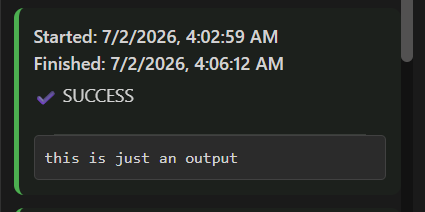
\includegraphics[width=0.5\textwidth]{images/workflow-page/workflow-text-image.png}
    \caption{Execution History Text Output Image}
\end{figure}
\begin{figure}[H]
    \centering
    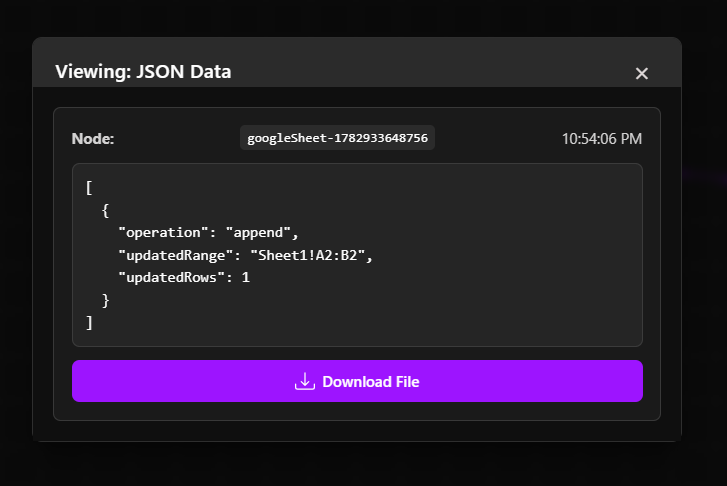
\includegraphics[width=0.5\textwidth]{images/workflow-page/workflow-json-image.png}
    \caption{Execution History Json Output Image}
\end{figure}
\begin{figure}[H]
    \centering
    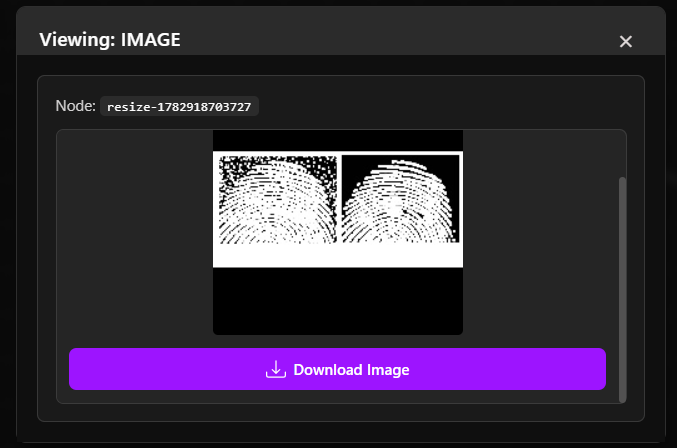
\includegraphics[width=0.5\textwidth]{images/workflow-page/workflow-image-image.png}
    \caption{Execution History Image Output Image}
\end{figure}
\begin{figure}[H]
    \centering
    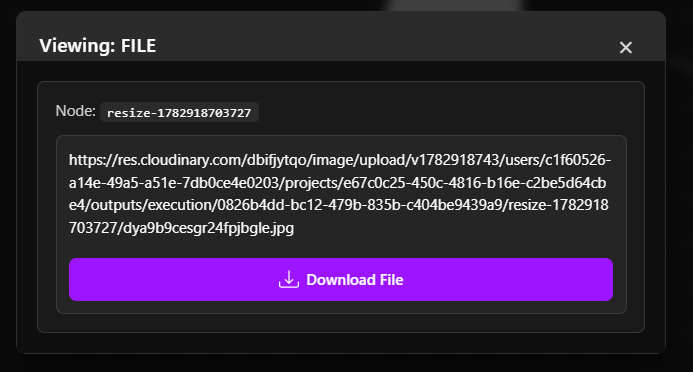
\includegraphics[width=0.5\textwidth]{images/workflow-page/workflow-file-image.png}
    \caption{Execution History File Output Image}
\end{figure}